\subsection{Grundlagen}
Gegeben sei eine Menge $S$ von $n$ Punkten in der Ebene und das Voronoi-Diagramm $V(S)$ der Menge.

Wie~\citeauthor{klein2005algorithmischegeometrie} schreibt, handelt es sich bei einer \textbf{\textit{Delaunay-Zerlegung}} $DT(S)$ um eine Menge von Liniensegmenten, welche bestimmte Bedingungen erfüllt. Diese entsteht durch die Verbindung zweier Puntke $p,q \in S$ zum Liniensegment $pq$, wenn die Voronoi-Regionen der Punkte $VR(p,S)$ und entsprechend $VR(q,S)$ an eine gemeinsame Voronoi-Kante $V(S)$ angrenzen. Das Liniensegment $pq$ heisst \textbf{Delaunay-Kante} (\citeyear[S. 231]{klein2005algorithmischegeometrie}).

\newpage

\begin{figure}[h]
\centering
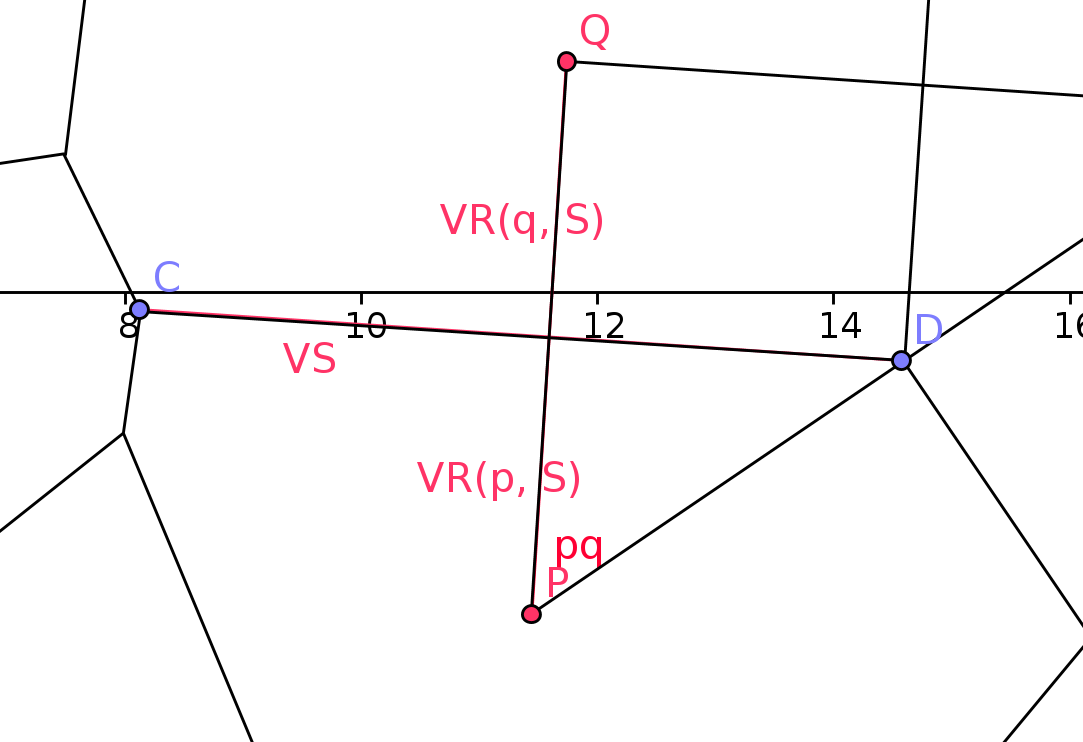
\includegraphics[width=200px]{images/delaunay_zerlegung_beispiel.png}
\caption{Beispiel einer Delaunay-Zerlegung\protect\footnotemark}
\label{fig:delaunayPartition}
\end{figure}
\footnotetext{Eigene Darstellung mittels Geogebra}

Da die \textbf{Delaunay-Triangulation} $\bm{DT(S)}$ eine kreuzungsfreie geometrische Realisierung des dualen Graphen des Voronoi-Diagramms ist, gilt also $DT(S) = V(S)^*$.
Daraus folgt, dass jede beschränkte Fläche der Delaunay-Zerlegung $DT(S)$ genau so viele Kanten hat, wie bei ihrem zugehörigen Knoten in $V(S)$ zusammen laufen.
Ist die Punktemenge $S$ so beschaffen, dass keine vier Punkte auf einem Kreisrand liegen, handelt es sich bei den beschränkten Flächen von $DT(S)$ um Dreiecke.
Aus diesem Grund heisst $DT(S)$ auch Delaunay-Triangulation der Punktemenge $S$~\parencite[S. 231 bis 237]{klein2005algorithmischegeometrie}.

\begin{minipage}[t]{0.3\textwidth}
    
\includegraphics[width=\textwidth]{images/delaunay_example_01_orig.png}
    \captionof{figure}{Originalbild\protect\footnotemark}
\label{fig:delaunayExample01Orig}
\end{minipage}
\footnotetext{\cite{imgur2012}}
\begin{minipage}[t]{0.3\textwidth}
    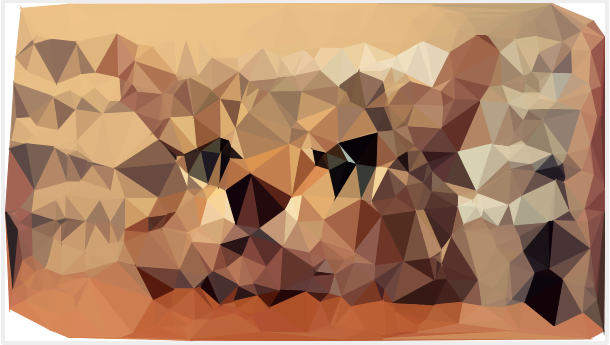
\includegraphics[width=\textwidth]{images/delaunay_example_01_500.png}
    \captionof{figure}{Triang. Bild aus 500 Punkten\protect\footnotemark}
\label{fig:delaunayExample01500}
\end{minipage}
\footnotetext{Eigene Darstellung mittels http://labs.vieron.net/delaunay-triangulations/}
\begin{minipage}[t]{0.3\textwidth}
    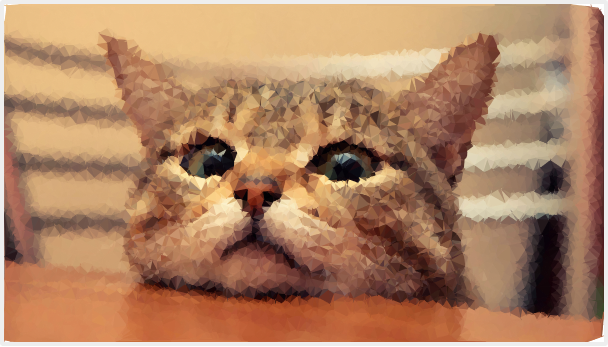
\includegraphics[width=\textwidth]{images/delaunay_example_01_8000.png}
    \captionof{figure}{Triang. Bild aus 8000 Punkten\protect\footnotemark}
\label{fig:delaunayExample018000}
\end{minipage}
\footnotetext{Eigene Darstellung mittels http://labs.vieron.net/delaunay-triangulations/}
